\documentclass[a4paper, 12pt, french]{article}
\usepackage[utf8]{inputenc}
\usepackage[T1]{fontenc}
\usepackage{babel}
\usepackage{setspace}
\usepackage{hyperref}
\usepackage{imakeidx}
\usepackage{graphicx}
\usepackage{fancyhdr}
\usepackage{chngcntr}
\usepackage{pifont}
\usepackage{xcolor}
\usepackage{glossaries}
\usepackage{helvet}
\usepackage{titlesec}
\usepackage{tikz}
\usepackage{rotating}
\usepackage{lscape}
\usepackage{wrapfig}
\usepackage[stable]{footmisc}

\makeindex[intoc]
 
\counterwithin{figure}{section}
\counterwithin{table}{section}

\definecolor{ssiYellow}{RGB}{255,237,0}
\definecolor{ssiRed}{RGB}{231,0,14}
\definecolor{ssiBlack}{RGB}{18,18,13}

\newcommand{\bdot}{\item[\color{ssiYellow}\ding{108}]} 
\newcommand{\bdotoutlined}{\item[\color{ssiYellow}\ding{109}]}
\newcommand{\bsquare}{\item[\color{ssiYellow}\ding{110}]} 

\hypersetup{%
    pdfborder = {0 0 0}
}
\renewcommand{\familydefault}{\sfdefault}

\titleformat{name=\section}{\normalfont\Large\bfseries\color{ssiBlack}}{\color{ssiYellow}\rule[-1.35mm]{3em}{1.25em}{\color{white}\hspace{-1cm}\normalfont\Large\bfseries\thesection\hspace{15pt}}}{1em}{}[\color{ssiYellow}{\titlerule[4pt]}\vspace*{4pt}]
\titleformat{\subsection}{\normalfont\Large\bfseries\color{ssiBlack}}{\color{ssiRed}\rule[-1.35mm]{3em}{1.25em}{\color{white}\hspace{-1.3cm}\normalfont\Large\bfseries\thesubsection\hspace{10pt}}}{1em}{}[\color{ssiYellow}{\titlerule[3pt]}\vspace*{4pt}]
\titleformat{\subsubsection}{\normalfont\Large\bfseries\color{ssiBlack}}{\color{ssiYellow}\rule[-1.35mm]{3em}{1.25em}{\color{white}\hspace{-1.60cm}\normalfont\Large\bfseries\thesubsubsection\hspace{5pt}}}{1em}{}[\color{ssiYellow}{\titlerule[2pt]}\vspace*{4pt}]

\titleformat{name=\section,numberless=true}{\color{ssiBlack}\normalfont\Large\bfseries}{}{0em}{}[\color{ssiYellow}{\titlerule[4pt]}\vspace*{4pt}]
\titleformat{name=\subsection,numberless=true}{\color{ssiBlack}\normalfont\Large\bfseries}{}{0em}{}[\color{ssiYellow}{\titlerule[3pt]}\vspace*{4pt}]
\titleformat{name=\subsubsection,numberless=true}{\color{ssiBlack}\normalfont\Large\bfseries}{}{0em}{}[\color{ssiYellow}{\titlerule[2pt]}\vspace*{4pt}]

\sloppy

\pagestyle{fancy}
\fancyhf{}
\rhead{Informatique et réseaux}
\lhead{PINEAU Anthony}

\begin{document}
	\begin{titlepage}
		\begin{center}

			\tikz[remember picture,overlay] \node[opacity=0.3,inner sep=0pt] at (current page.center){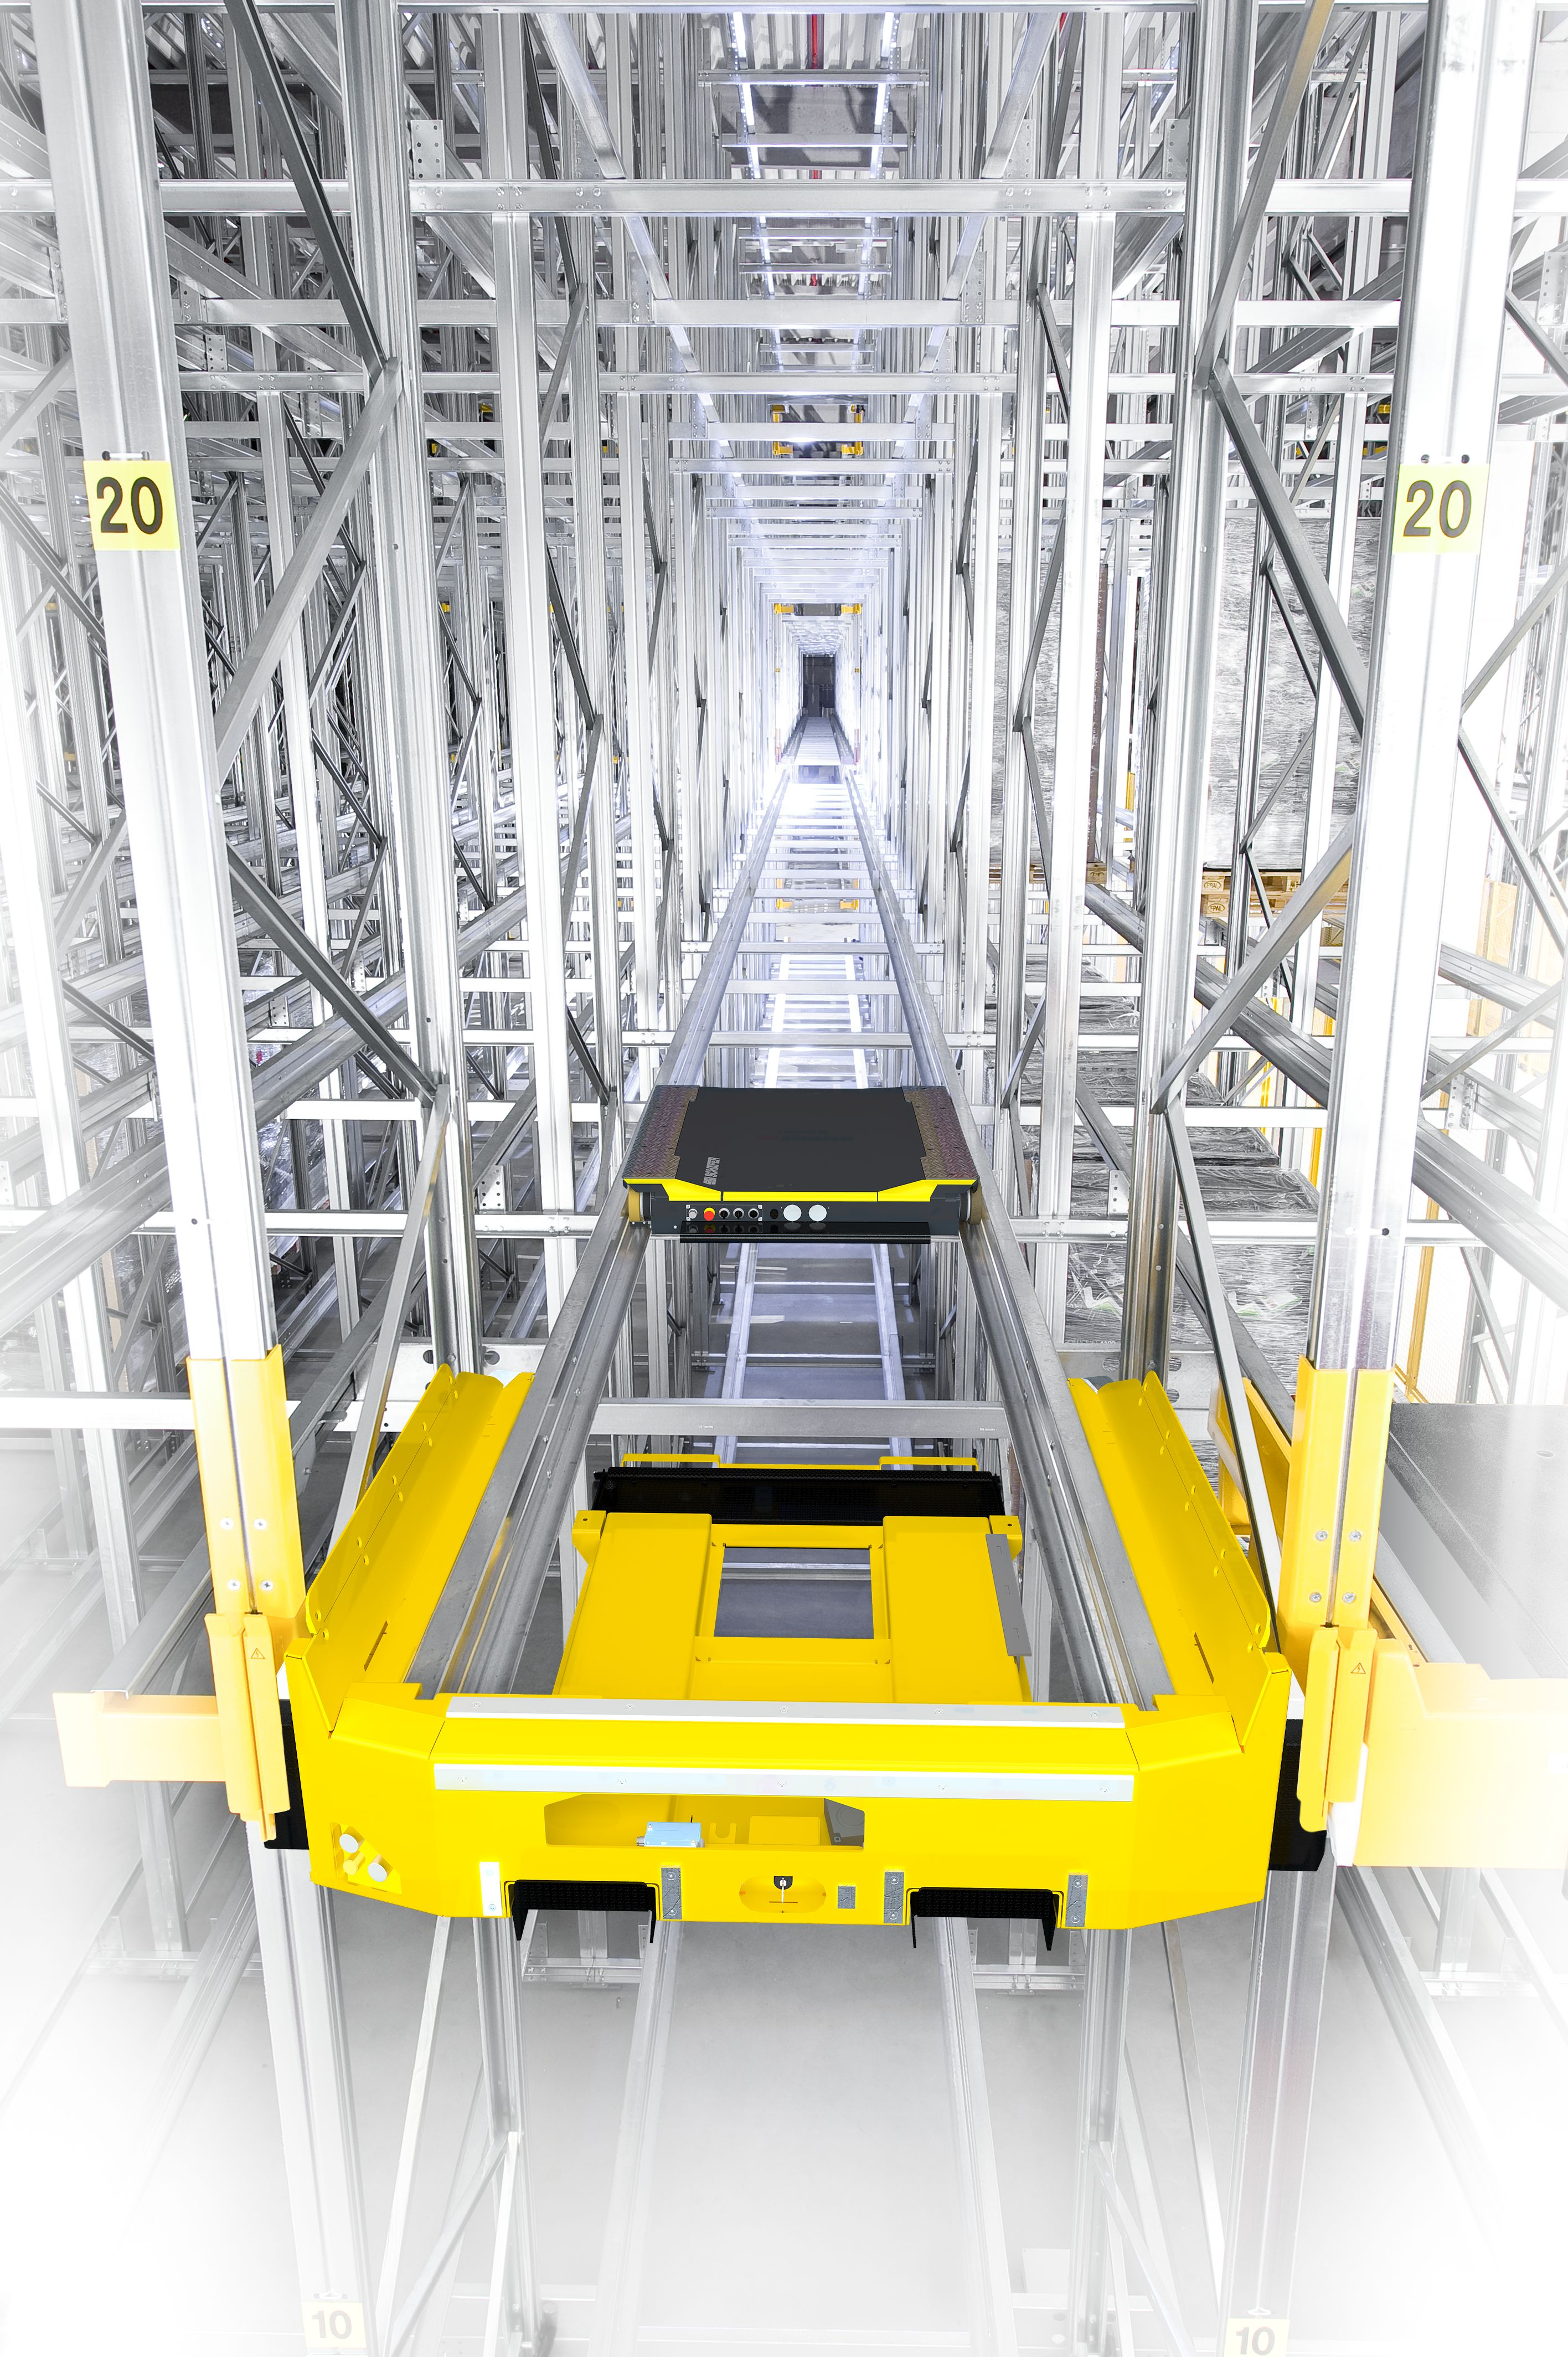
\includegraphics[width=\paperwidth,height=\paperheight]{../images/ssi_orbiter_highlight.jpg}};

			%\vspace*{1cm}

			\Huge
			\textbf{Rapport d'avancement}

			\vspace{0.5cm}
			\LARGE
			"Développement Delphi"

			\vspace{1.5cm}

			\textbf{Anthony PINEAU}\\
			\textbf{IR2023}

			\vfill

			
\includegraphics[width=0.6\textwidth]{../images/schaefer.jpg}
			\vfill
			
\includegraphics[width=0.4\textwidth]{../images/esaip.jpg}

			\vfill

			Période effectuée du\\
			13 mars 2023 au 14 avril 2023

			\vspace{0.8cm}
			
			\Large
			Maître de stage : Monsieur Thierry NEROT\\
			Tuteur pédagogique : Monsieur Sofiane HAMRIOUI\\
		\end{center}
	\end{titlepage}
		
	\newpage
	
	\doublespacing
	\tableofcontents

	\newpage
		
	\rfoot{Page \thepage}
	
	\phantomsection
	\listoffigures
	\addcontentsline{toc}{section}{\listfigurename}
	
	\newpage
	
	\singlespacing

	\phantomsection
	\section{Objectifs de la période et mise en évidence de tout changement stratégique}
	
	\newpage

	\section{Travaux réalisés}

	\newpage

	\section{Difficultés rencontrées}
	
	
	\newpage

	\section{Suite des travaux}
		
	\newpage

	\section{Mise à jour du planning du projet}

	\newpage
	
	\phantomsection
	\section*{Conclusion}
	\addcontentsline{toc}{section}{Conclusion}
	Pour conclure, j'ai effectué mon stage de deuxième année du cycle ingénieur du numérique à l'ESAIP en tant que stagiaire développeur au sein de l'entreprise SSI SCHÄFER. Lors de ce stage de deux mois, j'ai pu mettre en pratique mes connaissances et mes compétences acquises pendant mes précédentes années d’études et me suis à nouveau confronter aux exigences du monde du travail.\\

	%Tout d'abord cela à permis à l'entreprise de statuer sur l'utilisation d'Android Studio ou non ...\\

	Il m’aura permis d’élargir mes connaissances et compétences, et de faire de nouvelles rencontres professionnelles. De plus, j’ai pu travailler dans de très bonnes conditions de travail. J’ai aussi la chance de travailler sur un projet très intéressant. Par ailleurs, ce stage confirme mon envie de continuer mes études et ma vie professionnelle dans le domaine de l’informatique et plus précisément dans le développement.\\

	Je tiens par ailleurs à remercier à nouveau tous les acteurs ayant pris part à la réussite de mon stage, et tout particulièrement les membres de l’équipe avec qui j’ai travaillé et qui ont su m’accueillir et m’intégrer dans leurs rangs. Je suis donc très heureux d’avoir pu effectuer mon stage au sein de l'entreprise SSI SCHÄFER et suis ravi de pouvoir revenir pour effectuer mon stage de fin d'études l'année prochaine.
   

	\newpage

	\phantomsection
	\appendix% On passe aux annexes
	\section*{Annexes}
	\addcontentsline{toc}{section}{Annexes}
		%si moins de 26 annexes
		\renewcommand{\thesubsection}{\Alph{subsection}}
		\counterwithin{figure}{subsection}
		\counterwithin{table}{subsection}
		%sinon
		%\renewcommand{\thesubsection}{\Roman{subsection}}

		\subsection{Dates importantes de l'histoire SSI SCHÄFER}\label{appendix:history}
			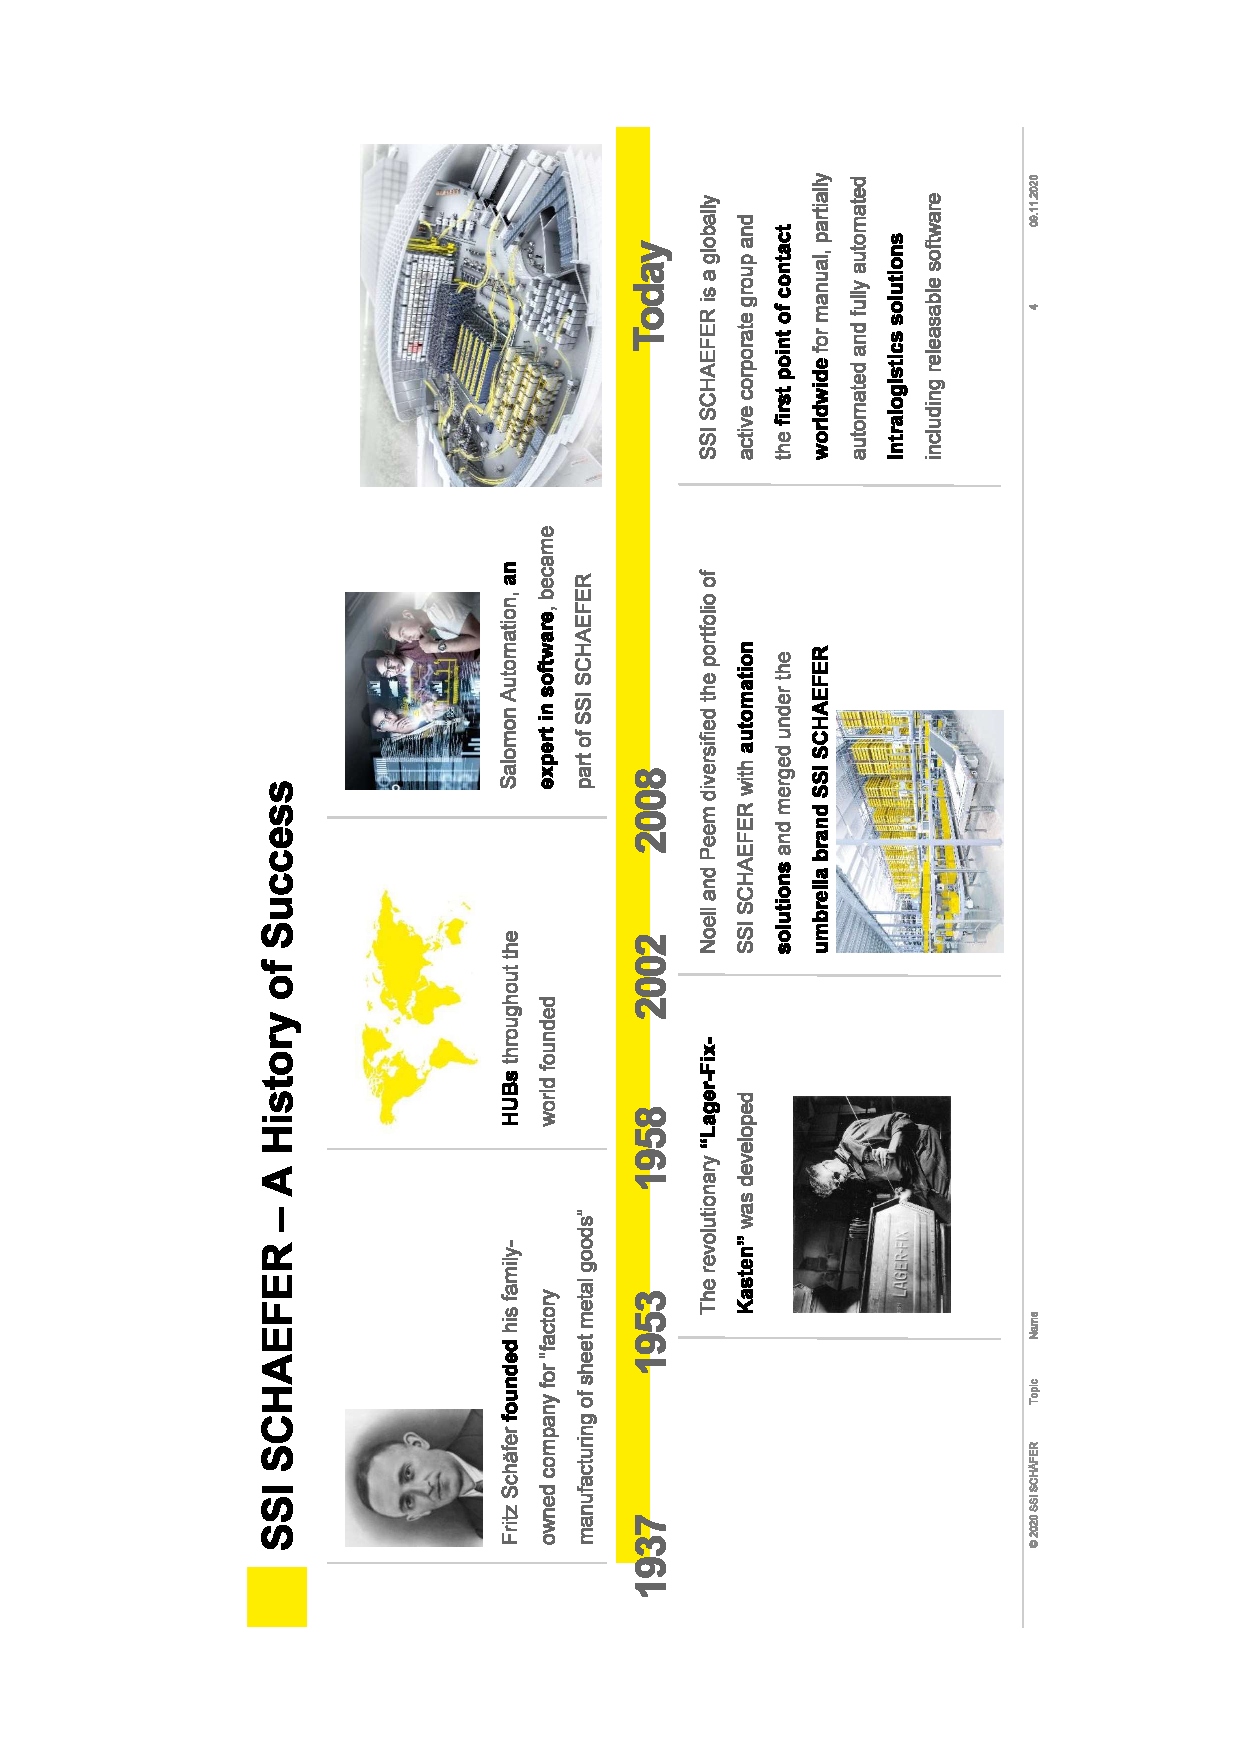
\includegraphics[width=0.8\linewidth]{../images/history.pdf}	

		\newpage

	\phantomsection
	\section*{Résumés}
	\addcontentsline{toc}{section}{Résumés}
		
\end{document}